\chapter{Methodology}
\label{chap:methodology}

\section{Overview}
\label{sec:meth:ov}

The problem defined in \autoref{chap:problem} is heavily behavior-driven. Model-based testing has excellent usage in describing behavior. With state machines, I could create a complete state space of the multiprotocol device.

I chose graphwalker as my modeling tool. It has a limited toolset for creating directed graphs, but it is a mature open-source package that can be used for MBT. The software can handle shared states that can synchronize multiple models. At its core, graphwalker is implemented in Java and only supports Maven projects natively. 

Since one of the goals was to create a project that runs on Python, more than graphwalker was needed. There is a Python package called altwalker, which acts as a Python wrapper around the executable and connects to graphwalker via internal sockets.

\autoref{sec:meth:sys_mod} details the modeling process and final artifacts created during the thesis work. The adaptor design is described in \autoref{sec:meth:ada}, and \autoref{sec:meth:ts} shows the entire test setup.

All the code and models developed for this thesis are publicly available on GitHub\cite{mis_github}.


\section{System modeling}
\label{sec:meth:sys_mod}

Graphwalker represents models as directed graphs. A graph node is called a vertex, and the edge is called an edge. Graphwalker recommends creating actions on edges and validating only on vertexes.

The Bluetooth Core specifies what a peripheral device shall be capable of. GAP defines discovery and connection mode as mandatory, leaving bonding, periodic advertising, and isochronous broadcast as excluded. Also, the LE Controller states that a minimal device shall be capable of scanning or advertising. After all, the set \[
    \{standby, scan, advertise, connected\}  
\] can describe the BLE device's state space. Since I am not testing the functionality of the profile - only the network capabilities - using any GATT services were not required.

<<figure ble>>

As 802.15.4 defines the whole association procedure, the Zigbee states should be \[
    \{disconnected, scan, association, joined\}
\]. Luckily, the application I was given had some plugins prepared for networking. The network-steering plugin automatically made the association process and gave its results. It tested the scanning, beaconing, and association procedures all in one. The final set of spaces is then reduced to just \[
    {disconnected, connected}
\]. Another plugin- throughput- was used to test the network's ability to relay data. The complete graph of Zigbee can be found in the following.

<<figure zigbee>>

For Thread, just as in Zigbee, the joining procedure is abstracted away.
The complete state space of a device is \[
    \{disabled, detached, child, router, leader\}  
\]. One of the limitations is that the application cannot stop the thread network; it just resets the stack. Since I am just creating a single-node network, having the router state is not relevant for this type of testing. With those two statements, the Thread state space is \[
    \{disabled, child\}  
\]. ICMP ping was used in the child state to test the connection.

<<figure thread>>

After creating the separate models, I could make the complete model for operating the three protocols side by side. Since graphwalker does not support regions or concurrently running multiple models, I combined the three models into one. The graph's vertexes could be described as \[
    \{standby, scan, advertise, peripheral\} \times  \{disconnected, joined\} \times \{disabled, child\}  
\]
\autoref{fig:meth_combined_model} shows the visual representation of the combined model.

\begin{figure}
    \centering
    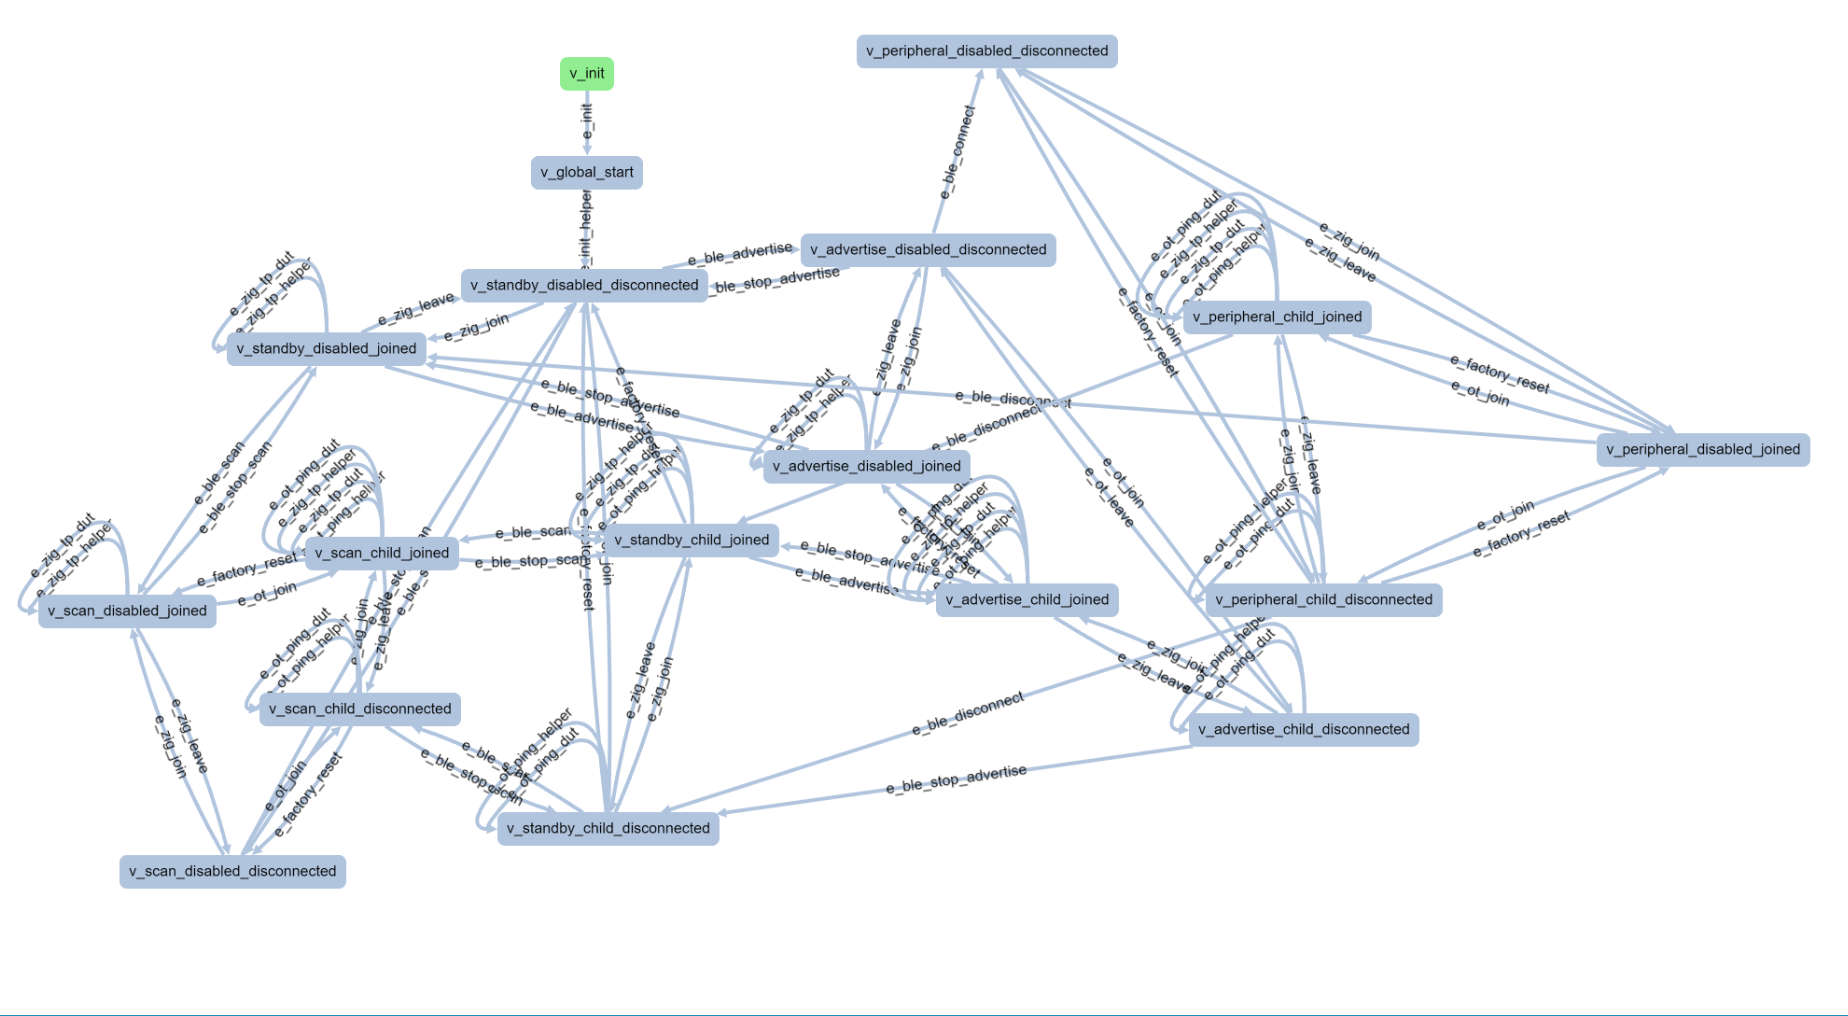
\includegraphics[width=150mm, keepaspectratio]{figures/combined_model.png}
    \caption{Combined protocol model}
    \label{fig:meth_combined_model}
\end{figure}


\section{Adaptation}
\label{sec:meth:ada}

An adaptor was needed to translate abstract test cases into concrete tests. Altwalker can create a template package from a given model. It has limitations regarding if a package already exists; it will fail to update the project. Creating models incrementally is beneficial. To solve this problem, I have created a simple utility that parses the package into a Python abstract syntax tree (AST). Then, the code will modify the AST to create missing methods. After the modifications, it will translate to Python syntax and save the file - leaving the old code intact.

To create the scenario defined in \autoref{chap:problem}, I needed to communicate with four different devices. Of those four, three were SoC applications, and I could use Silicon Labs' pyBgApi solution for the BLE helper.

The software architecture is divided into four layers. The highest level is the abstract device represented with contents in the interface package. It contains all the necessary functions a BLE, a Zigbee, and a Thread device shall do. The application package contains the concrete implementations of the interfaces.

The plugins package is the middleware for each application. It functions as a transport-free abstraction for commands. This allows commands to be independent of the underlying transport layer. If there is a new channel - let's say ssh - commands can be ported without any changes to the plugins.

Transportation was placed on the lowest layer. It represents the connection with the test-ware, the Silicon Labs' WPK main board. A link is abstracted behind the BaseTransport class. Different transport implementations are kept internal within the package. To help create a suitable transport for a device, I made the transport\_factory method that chose the matching transport for the given type. With this solution, it is possible to add new configurations for a device type easily.

A device can produce events asynchronously from the commands. For this, I made the telnet connection to listen on a separate thread. Furthermore, the plugins implement the observable pattern. It is possible to attach plugin handle methods to a transport, achieving asynchronous event handling.

The MpScenario class is responsible for initializing the applications. The package implements a singleton pattern. Test adaptors can access it via the get\_mp\_scenario function. This approach makes it possible to connect it to a multi-model test suite.

The whole architecture is shown in \autoref{fig:meth:arch}

\begin{figure}
    \centering
    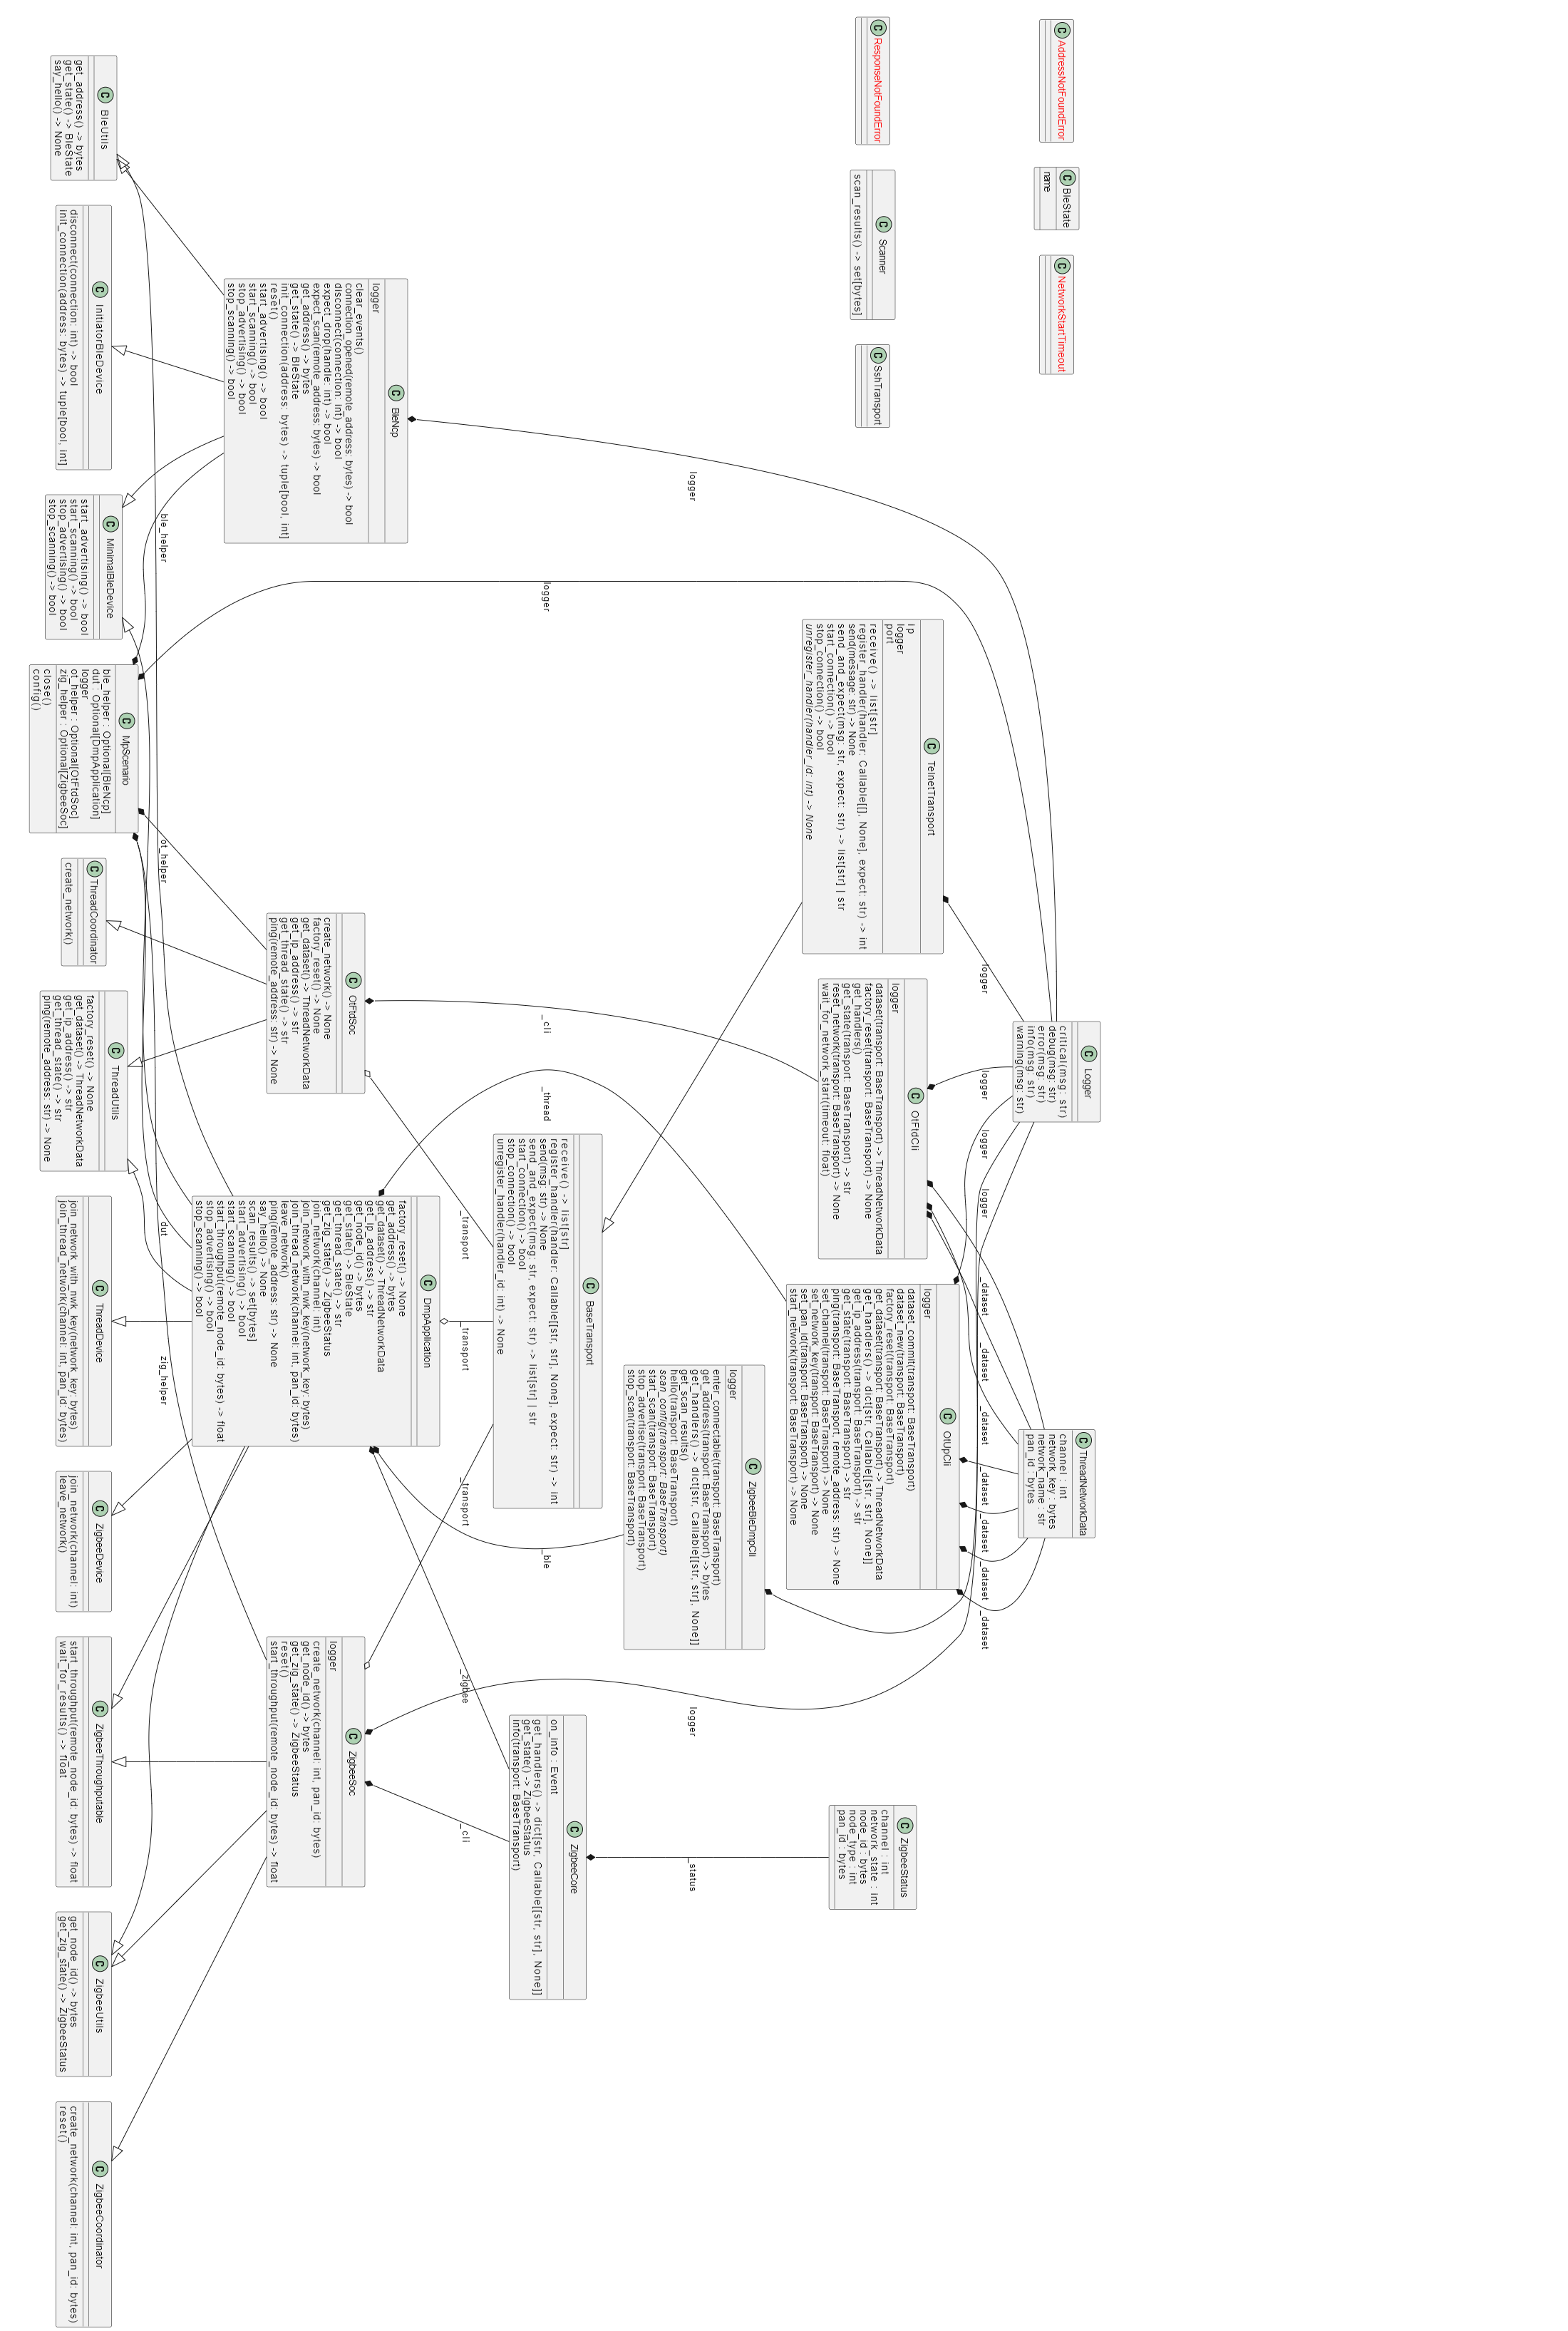
\includegraphics[width=140mm, keepaspectratio]{figures/classes.png}
    \caption{Adaptor architecture}
    \label{fig:meth:arch}
\end{figure}

\section{Test setup}
\label{sec:meth:ts}

I prepared a docker file that contains the adaptor code. It facilitates redistribution and ease of use. Docker is helpful because although altwalker is used, the test runner must also install graphwalker. Many companies have strict policies on what can be installed on company devices, and using docker is safe because it has a base image with graphwalker already installed.

The test setup consists of a test runner connected to a local network. Silicon Labs' WPKs are connected to the network as well. The test runner controls and monitors all the physical devices. <<figure>> shows the test setup overview.

<<figure test setup>>